\newcommand\tab[1][1cm]{\hspace*{#1}}

\chapter{Fonctionnalités}
\label{s:fonctionnalite}

\section{Image}
\subsection{Importation}
Non implémenté

\subsection{Exportation}
L'exportation en image est implémentée grâce à la méthode imageExport de la classe renderer. Tout d’abord, on dessin la scène, sans l’interface graphique. Ensuite, on sauvegarde une capture de l’écran avec le nom, un time stamp, pour que le fichier soit unique, et l’extension reçu en paramètre.

\begin{lstlisting}
void renderer::imageExport(const string name, const string extension)
{
	draw();
	
	ofImage imageTemp;
	
	// extraire des données temporelles formatées
	string timestamp = ofGetTimestampString("-%y%m%d-%H%M%S-%i");
	
	// générer un nom de fichier unique et ordonné
	string fileName = name + timestamp + "." + extension;
	
	// capturer le contenu du framebuffer actif
	imageTemp.grabScreen(0, 0, ofGetWindowWidth(), ofGetWindowHeight());
	
	// sauvegarder le fichier image
	imageTemp.save(fileName);
	
	ofLog() << "<export image: " << fileName << ">";
}
\end{lstlisting}


\subsection{Espace de couleur}
 L'espace de couleur utilisé par l'application est le HSB. Ainsi, pour chaque couleur à saisir, trois «sliders» sont disposer dans l'interface pour saisir la teinte (Hue), la saturation (Saturation) et la valeur (Brightess).
 
 En soit, à chaque mise à jours de l'application, l'application met à jours les valeurs des attributs de couleur dans la classe renderer. Ainsi, à chaque instant, le renderer a les couleurs entrées par l'utilisateur.
 
 Voici un exemple d'initiation des valeurs pour la couleur de remplissage:
 \begin{lstlisting}
 	fillHue.setName("Teinte");
 	fillHue.setMin(0);
 	fillHue.setMax(255);
 	fillHue.set(0);
 
 	fillSaturation.setName("Saturation");
 	fillSaturation.setMin(0);
 	fillSaturation.setMax(255);
 	fillSaturation.set(100);
 
 	fillBrightess.setName("Valeur");
 	fillBrightess.setMin(0);
	fillBrightess.setMax(255);
	fillBrightess.set(255);
 
 	fillAlpha.setName("Transparence");
 	fillAlpha.setMin(0);
 	fillAlpha.setMax(255);
 	fillAlpha.set(255);
 \end{lstlisting} 

Voici la méthode qui génère les couleurs à partir de l'espace HSB:
\begin{lstlisting}
	void ofApp::setColors()
	{
		stroke = ofColor::fromHsb(strokeHue, strokeSaturation, strokeBrightess, strokeAlpha);
		fill = ofColor::fromHsb(fillHue, fillSaturation, fillBrightess, fillAlpha);
		background = ofColor::fromHsb(bgHue, bgSaturation, bgBrightess);
	}
\end{lstlisting} 

Voici la méthode qui met à jours les couleurs du renderer (et l'épaisseur de lignes):
\begin{lstlisting}
	void ofApp::setRendererParameter() {
		
		rend->stroke = stroke;
		rend->fill = fill;
		rend->background = background;
		
		rend->strokeThickness = strokeThickness;
	}
\end{lstlisting}


\subsection{Traitement d'image}
Une catégorie situé au coin droit de l’écran permet l’utilisation de plusieurs filtres s’affichant sur l’entièreté de la scène. Elle regroupe trois type de filtres: le brouillage (Blur), l’inversement des couleurs et la dilatation. Les trois filtres peuvent être appliqués tous en même temps ou un à la fois.\\

Un objet ofxCvColorImage est utilisé pour la réalisation des filtres. On capture les pixels de la scène et on l’ajoute dans cet objet, pour ensuite lui faire subir les filtres sélectionnés par l’utilisateur. Les fonctions blur(), invert() et dilate() on été utilisées pour construire le filtre. Ces fonctions utilisent différentes opérations sur chaque pixel de l’image pour les modifier.\\

Voici une image d’une scène avec des filtres d’inversement de couleurs et de brouillage:\\
\begin{figure}[h]
	\centering
	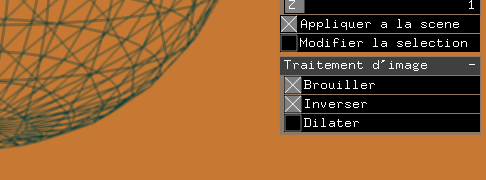
\includegraphics[width=5cm]{fig/filters.png}
	\caption{Une scène avec filtres.}
	\label{fig:filtres}
\end{figure}


\subsection{Image procédurale}
Non implémenté

\newpage

\section{Dessin vectoriel}

\subsection{Curseur dynamique}

Dans notre application il y a une interface graphique créée avec ofxGui. Cette technologie, malgré le fait qu'elle soit très pratique pour nos besoins, contient des boutons, des cases à cocher, des "sliders", des groupes, mais le curseur était toujours identique (en forme de flèche), ce qui ne rendait pas évident avec quoi on peut ou ne peut pas interagir.

Nous avons donc ajouté, en utilisant les événements mouseMoved() de notre fenêtre et des différents contrôles, une modification dynamique du curseur selon au dessus de quoi il se trouve.

Au a donc trois curseurs différents.

Le curseur normal, qui est présent quand la souris est dans l'espace de dessin

\begin{figure}[h]
	\centering
	\includegraphics[width=5cm]{fig/curseurNormal.png}
	\caption{Curseur normal de type "flèche"}
	\label{fig:test}
\end{figure}

Le curseur de type "main", qui est présent quand la souris est au dessus d'un bouton ou d'une case à cocher

\begin{figure}[h]
	\centering
	\includegraphics[width=5cm]{fig/curseurBouton.png}
	\caption{Curseur pour bouton de type "main"}
	\label{fig:test}
\end{figure}

Et le curseur de type "slider", qui est présent quand la souris est au dessus d'un contrôle du même nom.

\begin{figure}[h]
	\centering
	\includegraphics[width=5cm]{fig/curseurSlider.png}
	\caption{Curseur slider de type "slider"}
	\label{fig:test}
\end{figure}

\begin{lstlisting}
void ofApp::mouseMoved(int x, int y) {
	HCURSOR curs;
	if (!cursorIsInControl(x, y))
	{
		curs = LoadCursor(NULL, IDC_ARROW);
		SetCursor(curs);
	}
}
\end{lstlisting}

\begin{lstlisting}
bool ofxButton::mouseMoved(ofMouseEventArgs & args){

	HCURSOR curs;
	if (cursorIsInControl(args.x, args.y))
	{
		curs = LoadCursor(NULL, IDC_HAND);
		SetCursor(curs);
	}
	return ofxToggle::mouseMoved(args);
}
\end{lstlisting}

\begin{lstlisting}
template<typename Type>
bool ofxSlider<Type>::mouseMoved(ofMouseEventArgs & args){
	mouseInside = isGuiDrawing() && b.inside(ofPoint(args.x,args.y));
	
	HCURSOR curs;
	if (mouseInside)
	{
		curs = LoadCursor(NULL, IDC_SIZEWE);
		SetCursor(curs);
	}
	
	return mouseInside;
}
\end{lstlisting}

\subsection{Primitives vectorielles}

Dans les types de primitives disponibles, on trouve la catégorie 2D. En sélectionnant cette catégorie, on peut ainsi dessiner des carrés, des cercles (ellipses), des triangles, des lignes et des points. Toutes ces primitives sont affectés par la position, la taille, l’épaisseur de traits, la couleur de remplissage et de bordure ainsi que la texture passée par l’utilisateur.\\

Des objets ofPath sont utilisés pour tous les types de primitives 2d créés. Afin d’avoir une meilleure intégration à la scène, une casse générique de primitives 2d a été créer. Pour les différents types, différentes méthodes ont été conçues pour créer les primitives. Ces méthodes utilisent les méthodes ellipse(), circle(), rect(), triangle() et line(). Elles appliquent chaque propriété spécifiée par l’utilisateur. Après chaque ajout, on ajoute ensuite les primitives dans la scène.\\

Voici à quoi ressemble les différentes primitives 2D:\\
\begin{figure}[h]
	\centering
	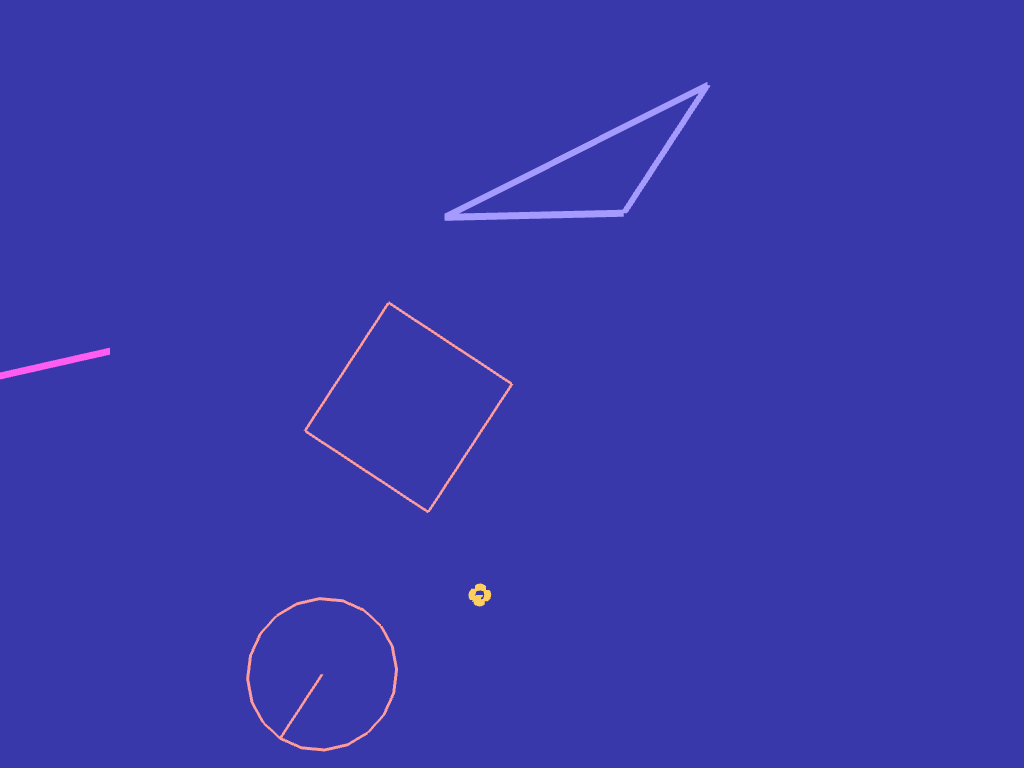
\includegraphics[width=5cm]{fig/primitives2d.png}
	\caption{Une scène avec primitives 2d.}
	\label{fig:prim2d}
\end{figure}

\subsection{Formes vectorielles}
La forme qui a été implémenté est un cornet de crème glacé, formé d'un cône et d'une sphère. Le code se trouve dans «renderer::createIceCream()» 

\begin{lstlisting}
ofParameter<bool>  renderer::createIcecream(int x, int y, int z, int sizeX, int sizeY, int sizeZ, ofColor color) {
	ofSpherePrimitive* ball = new ofSpherePrimitive();
	ball->setPosition(x, y + sizeY / 3, z);
	
	ofConePrimitive* cone = new ofConePrimitive();
	cone->setPosition(x, y - sizeY / 3, z);
	
	float smallestSphere = min(sizeX, min(sizeY, sizeZ));
	ball->setRadius(smallestSphere / 2);
	
	float smallestCone = min(sizeX, sizeZ);
	cone->setRadius(smallestCone / 2);
	cone->setHeight(sizeY);
	
	float newX = (float)sizeX / smallestSphere;
	float newY = (float)sizeY / smallestSphere;
	float newZ = (float)sizeZ / smallestSphere;
	
	ofMatrix4x4 matrix = ofMatrix4x4();
	matrix.scale(newX, newY, newZ);
	matrix.setTranslation(x, y, z);
	
	forme3d forme{ ball, color, matrix };
	forme.addPrimitive(cone);
	forme.setName("IceCream " + to_string(scn->nbElements() + 1));
	scn->addElement(forme);
	return forme.selected;
}
\end{lstlisting}

\begin{figure}[h]
	\centering
	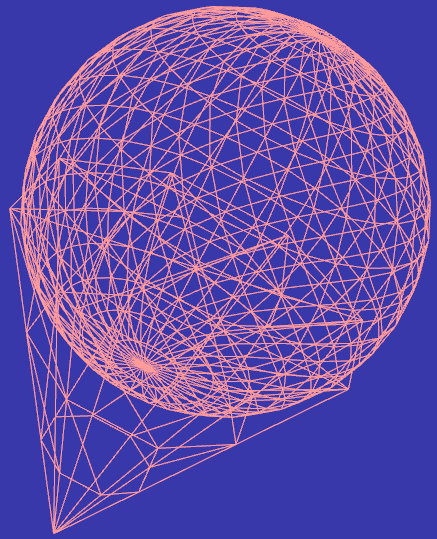
\includegraphics[width=5cm]{fig/iceCream.png}
	\caption{Cornet de crème glacé!}
	\label{fig:iceCream}
\end{figure}

On aurait bien voulu le faire avec des primitives 2D, mais on s'est dit qu'en 3D ça amenait un peu plus de défi!

\subsection{Outils de dessin}
L'outil de dessin a été implémenté en ajoutant des «sliders» dans l'interface afin de pouvoir modifier la couleur de remplissage, la couleur du contour, la couleur d'arrière plan et l'épaisseur des lignes de contour. Ainsi, il possible de modifier en tout temps la couleur d'arrière plan ou bien de modifier la couleur de remplissage, la couleur de contour et l'épaisseur des lignes de contour pour la création de primitive.

En pratique, à chaque mise à jour de l'application, les valeurs des attributs de la classe renderer sont mises à jour. Ainsi, les valeurs de couleurs ou d'épaisseur des lignes sont à jour lors de la création d'une primitive, tout comme la couleur d'arrière plan est à jour lorsque l'arrière plan est redéssiné.  

Voici la méthode qui met à jours les couleurs et l'épaisseur de lignes du renderer:
\begin{lstlisting}
	void ofApp::setRendererParameter() {
		
		rend->stroke = stroke;
		rend->fill = fill;
		rend->background = background;
		
		rend->strokeThickness = strokeThickness;
	}
\end{lstlisting}

Voici la méthode qui affiche à l'écran le contenu du renderer. La première ligne consiste a déssiner l'arrière plan:
\begin{lstlisting}
	void renderer::draw()
	{
		ofClear(background);
		
		[...]
	}
\end{lstlisting}

Voici une des méthodes qui ajoute une primitive à la scène. Les paramètres «fill» et «stroke» utilisé ici sont les attributs de couleurs de remplissage et de contour de la classe renderer:
\begin{lstlisting}
	ofParameter<bool> renderer::createSquare(float x, float y, float w, float h) {
		return createSquare(x,y,w,h,fill, stroke);
	}
\end{lstlisting}

\subsection{Interface}
L'application est dotée d'une interface utilisateur qui permet de modifier les paramètres d'une primitive à ajouter, ajouter une primitive à la scène, vider la scène, modifier les paramètres de la caméra, appliquer des transformations sur les primitives ou sur la scène, appliquer des effets de traitement d'image, sélectionner des primitives à l'aide d'une liste à cocher, importer un modèle 3D, exporter en image et quitter. 

L'interface a été développé avec «l'addons» ofxGui. Ainsi, nous avons créé des «panels» (ofxPanel) dans lesquels les différents paramètres de l'application ont été ajouté et «l'addons» se chargeait de générer les «sliders» et les cases à cocher associées aux paramètres. Nous avons aussi pu ajouté des boutons (ofxButton).

Comme l'essentiel du code de la classe qui gère l'interface représente plus de 1000 lignes, seulement quelques exemples seront montrés afin d'allégé ce document.

Voici l'initialisation de paramètres:
\begin{lstlisting}
void ofApp::initOfParameters() 
{
	[...]
	
	primPosX.setName("X");
	primPosX.setMin(MinX);
	primPosX.setMax(MaxX);
	primPosX.set((MinX + MaxX) / 2);
	
	primPosY.setName("Y");
	primPosY.setMin(MinY);
	primPosY.setMax(MaxY);
	primPosY.set((MinY + MaxY) / 2);
	
	primPosZ.setName("Z");
	primPosZ.setMin(MinZ);
	primPosZ.setMax(MaxZ);
	primPosZ.set((MinZ + MaxZ) / 2);
	
	[...]
}
\end{lstlisting}

Voici l'initialisation de groupes de paramètres (ofParameterGroup):
\begin{lstlisting}
void ofApp::initGroups()
{
	[...]
	
	groupPrimitivePosition2D.setName("Position");
	groupPrimitivePosition2D.add(primPosX.set(primPosX));
	groupPrimitivePosition2D.add(primPosY.set(primPosY));
	
	groupPrimitivePosition3D.setName("Position");
	groupPrimitivePosition3D.add(primPosX.set(primPosX));
	groupPrimitivePosition3D.add(primPosY.set(primPosY));
	groupPrimitivePosition3D.add(primPosZ.set(primPosZ));
	
	[...]
}
\end{lstlisting}

Voici la configuration de menu:
\begin{lstlisting}
void ofApp::setupMenu2D() {

	menu2D.setDefaultWidth(200);
	
	menu2D.setup();
	
	menu2D.add(groupPrimitiveType2D);
	menu2D.add(groupPrimitivePosition2D);
	menu2D.add(groupPrimitiveSize2D);
	
	menu2D.add(groupThick);
	
	menu2D.add(groupFill);
	
	menu2D.add(groupStroke);
	
	menu2D.add(groupTexture);
	
	menu2D.minimizeAll();
	
	menu2D.registerMouseEvents();
}
\end{lstlisting}

Voici la configuration des écouteurs sur les différents boutons de l'application:
\begin{lstlisting}
void ofApp::initButtonListener() {
	btnDrawPrimitive.addListener(this, &ofApp::btnDrawPrimitiveClicked);
	btnClear.addListener(this, &ofApp::btnClearClicked);
	btnExit.addListener(this, &ofApp::btnExitClicked);
	
	btnExport.addListener(this, &ofApp::btnExportClicked);
	btnImport.addListener(this, &ofApp::btnImportClicked);
	
	btnApplySelect.addListener(this, &ofApp::btnApplySelectClicked);

\end{lstlisting}

Voici la méthode setup de la classe ofApp:
\begin{lstlisting}
void ofApp::setup()
{
	[...]
	
	initOfParameters();
	initGroups();
	
	setupMenu2D();
	setupMenu3D();
	setupCameraMenu();
	setupTransformationMenu();
	setupOptionMenu();
	setupSelectionMenu();
	
	initButtonListener();
	
	[...]
}
\end{lstlisting}

Voici une capture d'écran pour montré l'interface:
\begin{figure}[h]
	\centering
	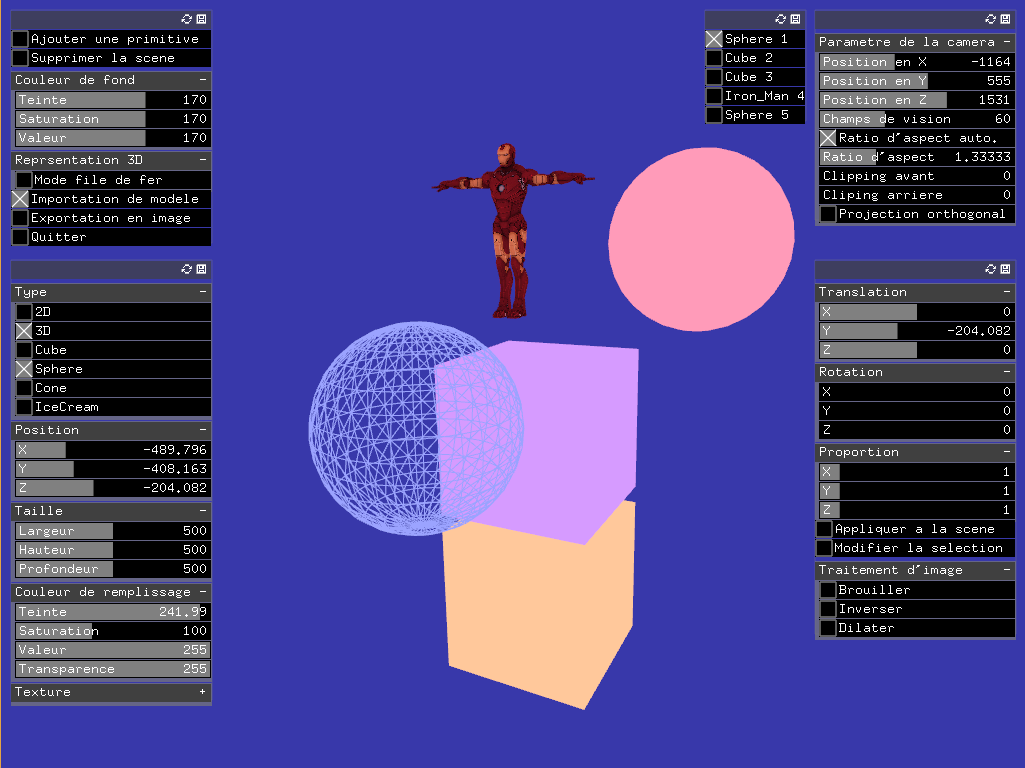
\includegraphics[width=15cm]{fig/InterfaceComplet.png}
	\caption{Exemple d'interface}
	\label{fig:interface}
\end{figure}

\pagebreak
\section{Transformation}
\subsection{Transformation interactive}
Une catégorie à droite de l’application permet de transformer le systèmes de coordonnées des entités géométriques de la scène. On peut exercer des transformations tel que la translation en X, Y et Z, la rotation en X, Y et Z ainsi que la proportion en X, Y et Z. Elle peut se faire autant en temps réel qu’en différé. \\

Les matrices de transformation d’openframeworks sont utilisés pour la réalisation des transformations. On utilise les méthodes ofPushMatrix() et ofPopMatrix(). Une fois la matrice empilé, on ajoute les transformation à l’aide des méthodes ofTranslate(), ofRotate() et ofScale() selon les paramètres inscrit par l’utilisateur. Enfin, on dépile la matrice pour permettre la transformation.\\

Voici le menu des transformations et ces différentes options:\\
\begin{figure}[h]
	\centering
	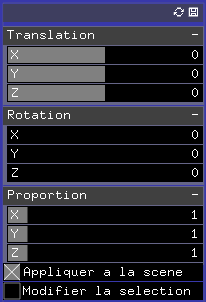
\includegraphics[width=5cm]{fig/transformations.png}
	\caption{Menu des transformations.}
	\label{fig:transformations}
\end{figure}

\subsection{Structure de scène}
La structure de scène a été implémenté sous la forme d'un arbre ordoné, dans lequel les feuilles sont les éléments de la scène. La classe scène comprend 4 classes interne, soit element, group, node et scene\_iterator. Les classes group et node héritent d'element et  servent à stocker tout ce qui se trouve dans la scène. La classe scene\_iterator permet, quant-à elle, de parcourir les éléments pour les dessiner. \\

On utilise les shared\_ptr au lieux des simples pointeurs pour conserver les éléments qui sont ajouté à la scène pour ne pas avoir à trop gérer la mémoire.\\

L'essentiel du code de la scène se trouve dans les méthodes addElement de la scène, des sous-clases de stockage et l'operator++ de l'itérateur.\\

\begin{lstlisting}
void scene::addElement(size_t index, primitive_ptr& p, bool insertFirstChild) {
	if (index == 0 && !insertFirstChild {
		throw invalid_argument("root don't have parent...");
	}
	root->addElement(index, p, insertFirstChild);
}

//Retourne la quantite d'element ajoute
size_t scene::node::addElement(size_t index, primitive_ptr& p, bool insertFirstChild) {
	if (index != this->index) {
		throw invalid_argument("index need to be equals to the index of the node");
	}
	if (insertFirstChild) {
		throw invalid_argument("node need to be wraped in a group");
	}
	this->content = p;
	contentType = "primitive";
	return 1;
}

//Retourne la quantite d'element ajoute
size_t scene::group::addElement(size_t index, primitive_ptr& p, bool insertFirstChild) {
	size_t addedSize = 0;
	
	if (this->index == index) {
		if (insertFirstChild) {
			//Inserer comme premier element
			childrens.insert(childrens.begin(), element_ptr{ new node{ index + 1, height + 1, p } });
			for (auto& it = childrens.begin() + 1; it < childrens.end(); ++it) {
				it->get()->setIndex(it->get()->getIndex() + 1);
			}
			addedSize++;
		} else {
			throw invalid_argument("element must to be add in the parent");
		}
	} else {
		size_t ubound = childrens.size();
		size_t lbound = 0;
		size_t i;
		
		//Recherche binaire
		while (lbound <= ubound) {
			i = lbound + (ubound - lbound) / 2;
			if (childrens[i]->getIndex() == index) {
				if (insertFirstChild) {
					if (childrens[i]->getType() != "group") {
						group_ptr temp = group_ptr{ new group{ index, height + 1 } };
						temp->childrens.push_back(childrens[i]);
						temp->childrens[0]->setIndex(index + 1);
						temp->childrens[0]->setHeight(height + 2);
						temp->size = temp->childrens[0]->getSize() + 1;
						childrens[i] = temp;
						addedSize++;
					}
					addedSize += childrens[i]->addElement(index, p, insertFirstChild);
				} else {
					childrens.insert(childrens.begin() + i + 1, element_ptr{ new node{ index + childrens[i]->getSize(), height + 1, p } });
					i++;
					addedSize++;
				}
				i++;
				break;
			} else if (childrens[i]->getIndex() < index) {
				lbound = i + 1;
				if (ubound < lbound) {
					//Ajoute l'element dans le groupe sous-jacent
					addedSize += childrens[i]->addElement(index, p, insertFirstChild);
					i++;
					break;
				}
			} else {
				ubound = i - 1;
				if (ubound < lbound) {
					//Ajoute l'element dans le groupe sous-jacent
					addedSize += childrens[i - 1]->addElement(index, p, insertFirstChild);
					break;
				}
			}
		}	
		for (auto& it = childrens.begin() + i; it < childrens.end(); ++it) {
			it->get()->setIndex(it->get()->getIndex() + addedSize);
		}
	}
	size += addedSize;
	return addedSize;
}

//Avance jusqu'au prochain node
void scene::scene_iterator::operator++() {
	for (rootIndex; rootIndex <= root->getSize(); ++rootIndex) {
		element* elem = root->getElement(rootIndex);
		if (elem->getType() != "group" && elem->getType() != "root") {
			primitive_ptr ptr = (dynamic_cast<node*>(elem))->content;
			if (p != ptr) {
				p = ptr;
				break;
			}
		}
	}
	if (rootIndex > root->getSize()) {
		p = primitive_ptr{ nullptr };
	}
}
\end{lstlisting}
Comme vous avez sans-doute remarqué, l'ajout d'élément à la scène se fait récursivement, à l'index en paramètre. Le paramètre «insertFirstChild» indique s'il faut insérer l'élément comme le premier enfant de l'élément à l'index en paramètre. S'il est faux, on insère simplement le nouvel élément après l'index. Dans group::addElement, on utilise un algorithme de recherche binaire pour trouver dans ou après quel élément il faut ajouter le nouvel élément. L'operator++, quant à lui, parcours la scène en s'arrêtant seulement sur les classes node. \\

Malheureusement, par manque de temps la structure de scène n'est pas utilisé à sont plein potentiel et tous les éléments sont stocké dans le groupe à la racine de la scène. Il est tout de même possible de voir le résultat en changeant la ligne «\#define test 0» pour «\#define test 1» dans le fichier «main.cpp». Vous verrez alors le résultat de l'exécution des tests de la classe scene (principalement de l'ajout et de la supression d'élément), se trouvant à la fin de «scene.cpp». \\

\newpage

\subsection{Sélection multiple}

Dans notre application, toutes les entités géométriques, soit les primitives en 2D, les primitives en 3D et les modèles 3D importés du disque, apparaissent dans un menu avec un nom unique.

\begin{figure}[h]
	\centering
	\includegraphics[width=5cm]{fig/menuSelection.png}
	\caption{Menu de selection}
	\label{fig:test}
\end{figure}

À partir de là, il est possible d'en sélectionner un ou plusieurs.

\begin{figure}[h]
	\centering
	\includegraphics[width=5cm]{fig/menuSelectionPlusieurs.png}
	\caption{Plusieurs entités sélectionnées}
	\label{fig:test}
\end{figure}

\newpage

Lorsqu'on est pas en mode "Wireframe", les entités sélectionnées seront affichées en wireframe quand même, de façon à les identifier. Comme le mode wireframe existe surtout à des fins de débogage et pour des opérations précises, on n'est pas censé l'utiliser en permanence, c'est pourquoi ce n'est pas grave si dans ce mode on ne peut pas voir aussi bien quelles entités sont sélectionnées.

\begin{figure}[h]
	\centering
	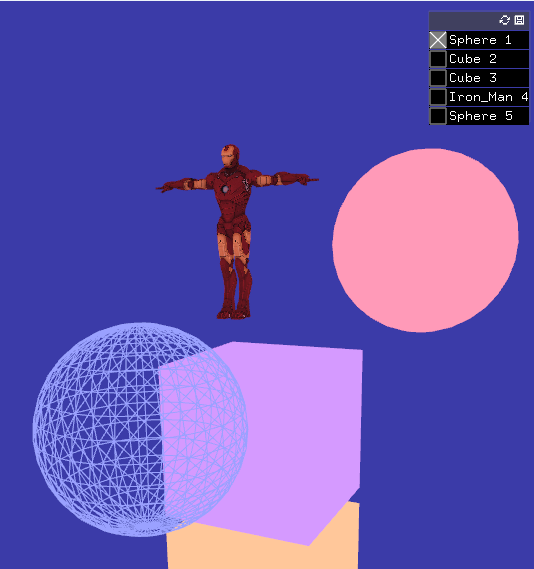
\includegraphics[width=12cm]{fig/WireframeSelection.png}
	\caption{La selection est en wireframe}
	\label{fig:test}
\end{figure}

\newpage

Les transformation géométriques peuvent être appliquées en même temps à toutes les entités sélectionnées, en appliquant une matrice de transformation à chacun d'entre eux en même temps. Cette matrice est créée à partir de "sliders", de translation, de rotation et de taille.

\begin{figure}[h]
	\centering
	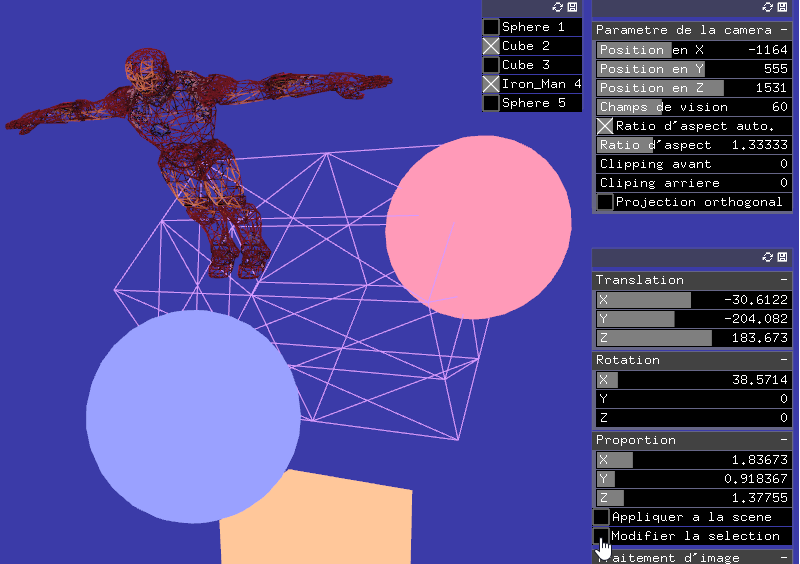
\includegraphics[width=18cm]{fig/transformationSelection.png}
	\caption{Chaque entité de la selection reçoit la transformation}
	\label{fig:test}
\end{figure}

\begin{lstlisting}

void renderer::applySelection(ofMatrix4x4 matrix)
{
	for (auto& p : *scn)
	{
		if (p.selected.get())
		{
			ofMatrix4x4 oldMat = p.getTransfo();
			p.setTransfo(oldMat * matrix);
		}
	}
	std::list<extModel>::iterator iterator4;
	for (iterator4 = externalModels.begin(); iterator4 != externalModels.end(); ++iterator4)
	{
		if (iterator4->selected.get())
		{
			ofMatrix4x4 oldMat = iterator4->getTransfo();
			iterator4->setTransfo(oldMat * matrix);
		}
	}
}
\end{lstlisting}

\begin{lstlisting}

void primitive3d::draw(bool wireframe) {

	ofPushMatrix();
	ofTranslate(transfoMatrix.getTranslation());
	
	ofSetColor(fillCol);
	
	ofQuaternion rotation = transfoMatrix.getRotate();
	float rotationAmount;
	ofVec3f rotationAngle;
	rotation.getRotate(rotationAmount, rotationAngle);
	
	ofRotate(rotationAmount, rotationAngle.x, rotationAngle.y, rotationAngle.z);
	
	ofScale(transfoMatrix.getScale());
	
	if (wireframe || selected.get())
	prim->drawWireframe();
	else
	prim->drawFaces();
	
	ofPopMatrix();
}

\end{lstlisting}

\subsection{Coordonnées non-cartésiennes}
Non-implémenté

\subsection{Historique}
Non-implémenté

\pagebreak
\section{Géométrie}
\subsection{Particules}
Non-implémenté

\newpage

\subsection{Primitives}

Dans notre application, il est possible de créer à partir d'algorithmes seulement plusieurs primitives en 3D. Ces primitives sont le cube, la sphère et le cône. Chaque primitive peut être créée directement avec une position et taille choisie par l'utilisateur, mais ces attributs pourront bien évidemment être modifiées par la suite (voir la section 4.3.3 sur la sélection multiple.).\\

On ne peut pas créer les primitives avec une rotation dès le départ, car ce n'est pas pertinent de donner une rotation à un objet comme un cône, quand il n'y aucun moyen de savoir quel est son orientation "sans rotation" avant d'en avoir créé un de toute façon. Il faut leur donner la rotation voulue après les avoir créées.\\

On peut aussi choisir une couleur par primitive, dans l'espace de couleur HSB.

\begin{figure}[h]
	\centering
	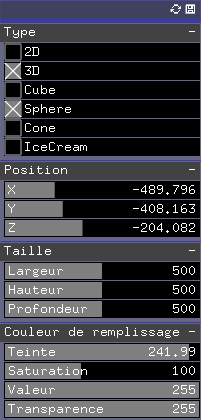
\includegraphics[width=6cm]{fig/creationPrimitive.png}
	\caption{Options de création d'une primitive}
	\label{fig:test}
\end{figure}

\newpage

\begin{lstlisting}
void ofApp::btnDrawPrimitiveClicked()
{
	ofLog() << "<app::btnDrawPrimitiveClicked>";
	
	if (primType2D.get()) {
		if (primTypeCube.get()) {
			selectionMenu.add(rend->createSquare(primPosX, primPosY, primSizeWidth, primSizeHeight));
		}
		else if (primTypeSphere.get()) {
			selectionMenu.add(rend->createCircle(primPosX, primPosY, primSizeWidth, primSizeHeight));
		}
		else if (primTypeTriangle.get()) {
			selectionMenu.add(rend->createTriangle(primPosX, primPosY, primPosX + primSizeWidth, primPosY, (primPosX + primSizeWidth) / 2, primPosY + primSizeHeight));
		}
		else if (primTypeLine.get()) {
			selectionMenu.add(rend->createLine(primPosX, primPosY, primSizeWidth, primSizeHeight));
		}
		else if (primTypePoint.get()) {
			selectionMenu.add(rend->createPoint(primPosX, primPosY, strokeThickness));
		}
	}
	else {
		if (primTypeCube.get()) {
			selectionMenu.add(rend->createCube(primPosX, primPosY, primPosZ, primSizeWidth, primSizeHeight, primSizeDepth));
		}
		else if (primTypeSphere.get()) {
			selectionMenu.add(rend->createSphere(primPosX, primPosY, primPosZ, primSizeWidth, primSizeHeight, primSizeDepth));
		}
		else if (primTypeTriangle.get()) {
			selectionMenu.add(rend->createCone(primPosX, primPosY, primPosZ, primSizeWidth, primSizeHeight, primSizeDepth));
		}
		else {
			selectionMenu.add(rend->createIcecream(primPosX, primPosY, primPosZ, primSizeWidth, primSizeHeight, primSizeDepth));
		}
	}
}
\end{lstlisting}

\newpage

\begin{lstlisting}
//-------------3D primitives-----------------------
ofParameter<bool> renderer::createCube(int x, int y, int z, int w, int h, int d)
{
	return createCube(x, y, z, w, h, d, fill);
}

ofParameter<bool> renderer::createCube(int x, int y, int z, int w, int h, int d, ofColor fillCol)
{
	ofBoxPrimitive* box = new ofBoxPrimitive();
	
	float smallest = min(w, min(h, d));
	
	box->setWidth(smallest);
	box->setHeight(smallest);
	box->setDepth(smallest);
	
	float newX = (float)w / smallest;
	float newY = (float)h / smallest;
	float newZ = (float)d / smallest;
	
	ofMatrix4x4 matrix = ofMatrix4x4();
	matrix.scale(newX, newY, newZ);
	matrix.setTranslation(x, y, z);
	
	for (int i = 0; i < 6; i++)
	{
		box->setSideColor(i, fillCol);
	}
	
	primitive3d prim = primitive3d{ box, fillCol, matrix };
	prim.setName("Cube " + to_string(scn->nbElements() + 1));
	scn->addElement(prim);
	return prim.selected;
	
	//cout << *scn;
}

ofParameter<bool> renderer::createSphere(int x, int y, int z, int sizeX, int sizeY, int sizeZ)
{
	return createSphere(x, y, z, sizeX, sizeY, sizeZ, fill);
}

ofParameter<bool> renderer::createSphere(int x, int y, int z, int sizeX, int sizeY, int sizeZ, ofColor color)
{
	ofSpherePrimitive* ball = new ofSpherePrimitive();
	ball->setPosition(0, 0, 0);
	
	float smallest = min(sizeX, min(sizeY, sizeZ));
	
	ball->setRadius(smallest/2);
	
	float newX = (float)sizeX / smallest;
	float newY = (float)sizeY / smallest;
	float newZ = (float)sizeZ / smallest;
	
	ofMatrix4x4 matrix = ofMatrix4x4();
	matrix.scale(newX, newY, newZ);
	matrix.setTranslation(x, y, z);
	
	primitive3d prim = primitive3d{ ball, color, matrix };
	prim.setName("Sphere " + to_string(scn->nbElements() + 1));
	scn->addElement(prim);
	return prim.selected;
}

ofParameter<bool> renderer::createCone(int x, int y, int z, int sizeX, int sizeY, int sizeZ)
{
	return createCone(x, y, z, sizeX, sizeY, sizeZ, fill);
}

ofParameter<bool> renderer::createCone(int x, int y, int z, int sizeX, int sizeY, int sizeZ, ofColor color)
{
	ofConePrimitive* cone = new ofConePrimitive();
	cone->setPosition(0, 0, 0);
	
	float smallest = min(sizeX, sizeZ);
	cone->setRadius(smallest / 2);
	cone->setHeight(sizeY);
	
	float newX = (float)sizeX / smallest;
	float newY = 1.0f;
	float newZ = (float)sizeZ / smallest;
	
	ofMatrix4x4 matrix = ofMatrix4x4();
	matrix.scale(newX, newY, newZ);
	matrix.setTranslation(x, y, z);
	
	primitive3d prim = primitive3d{ cone, color, matrix };
	prim.setName("Cone " + to_string(scn->nbElements() + 1));
	scn->addElement(prim);
	return prim.selected;
	
}
\end{lstlisting}

\subsection{Modèle}

Il est possible pour un utilisateur d'importer un modèle choisit sur son ordinateur. Les modèles supportés sont ceux qui ont un des formats suivants:

\begin{list}{}{}
	\item 3DS \tab ASE \tab DXF \tab HMP \tab MD2 \tab MD3
	\item MD5 \tab MDC \tab MDL \tab NFF \tab PLY \tab STL 
	\item X \tab LWO \tab OBJ \tab SMD \tab Collada \tab LWO
	\item Ogre XML \tab partly LWS
\end{list}

\begin{figure}[h]
	\centering
	\includegraphics[width=6cm]{fig/importerModele.png}
	\caption{Bouton pour importer un modèle}
	\label{fig:test}
\end{figure}

Si le modèle est dans un répertoire avec ses textures dans le bon chemin relatif, celles-ci seront automatiquement chargées et appliquées. De plus, si l'importation du modèle échoue pour une quelconque raison, un message sera affiché à l'utilisateur pour l'informer.\\

Un modèle peut être sélectionné comme une primitive, sera affecté par le mode "Wireframe", et sera modifié si on applique une matrice de transformation pendant qu'il est sélectionné.

Une partie du code qui suit vient de MSDN (Microsoft), dont le lien peut-être trouvé dans la section Références. Nous avons modifié le code pour qu'il convienne à nos besoins.

\begin{lstlisting}
void ofApp::btnImportClicked()
{
	HRESULT hr = CoInitializeEx(NULL, COINIT_APARTMENTTHREADED |
	COINIT_DISABLE_OLE1DDE);
	if (SUCCEEDED(hr))
	{
		IFileOpenDialog *pFileOpen;
		
		// Create the FileOpenDialog object.
		hr = CoCreateInstance(CLSID_FileOpenDialog, NULL, CLSCTX_ALL,
		IID_IFileOpenDialog, reinterpret_cast<void**>(&pFileOpen));
		
		if (SUCCEEDED(hr))
		{
			// Show the Open dialog box.
			hr = pFileOpen->Show(NULL);
			
			// Get the file name from the dialog box.
			if (SUCCEEDED(hr))
			{
				IShellItem *pItem;
				hr = pFileOpen->GetResult(&pItem);
				if (SUCCEEDED(hr))
				{
					LPWSTR pszFilePath;
					hr = pItem->GetDisplayName(SIGDN_FILESYSPATH, &pszFilePath);
					
					// Display the file name to the user.
					if (SUCCEEDED(hr))
					{
						
						std::wstring path = wstring(pszFilePath);
						std::string strPath(path.begin(), path.end());
						ofParameter<bool> param = rend->importModel(strPath);
						
						if (param.get() == false)
						{
							selectionMenu.add(param);
							strPath = "Le modele " + strPath + " a ete importe avec succes!";
							path = std::wstring(strPath.begin(), strPath.end());
							LPCWSTR title = (LPCWSTR)path.c_str();
							MessageBox(NULL, title, L"Succes", MB_OK);
						}
						else
						{
							strPath = "Le modele n'a pas pu etre importe.";
							path = std::wstring(strPath.begin(), strPath.end());
							LPCWSTR title = (LPCWSTR)path.c_str();
							MessageBox(NULL, title, L"Echec", MB_OK);
						}
						
						CoTaskMemFree(pszFilePath);
					}
					pItem->Release();
				}
			}
			pFileOpen->Release();
		}
		CoUninitialize();
	}
}
\end{lstlisting}

\begin{lstlisting}
ofParameter<bool> renderer::importModel(string path) {
	ofxAssimpModelLoader* model = new ofxAssimpModelLoader();
	bool ret = model->loadModel(path, false);
	if (ret)
	{
		model->enableTextures();
		ofTexture tex = ofTexture();
		extModel mod = extModel(model);
		
		string fName(path);
		size_t pos = fName.rfind(".");
		if (pos != string::npos)
		{
			if (pos != 0)
			{
				fName = fName.substr(0, pos);
			}
		}
		pos = fName.rfind("\\");
		if (pos != string::npos)
		{
			if (pos != 0)
			{
				fName = fName.substr(pos + 1);
			}
		}
		
		mod.setName(fName + " " + to_string(externalModels.size() + 1));
		scn->addElement(mod);
		return mod.selected;
	}
	return ofParameter<bool>(true);
}
\end{lstlisting}

\subsection{Texture}
Implémenté

\subsection{Géométrie procédurale}
Non-implémenté

\pagebreak
\section{Caméra}
\subsection{Propriétés de caméra}
Les propriétés de la caméra tel que le champ de vision, le ratio d'aspect ainsi que la distance du plan de clipping avant et arrière. Ils peuvent être modifier dans l'interface graphique à l'aide de slider. L'essentiel du code se trouve dans «ccamera::update()».


\begin{lstlisting}
	cam->setFov(fov.get());
	if (autoRatio.get()) {
		cam->setForceAspectRatio(false);
	} else {
		cam->setAspectRatio(ratio.get());
	}
	cam->setNearClip(nearClip.get());
	cam->setFarClip(farClip.get());
\end{lstlisting}

\begin{figure}[h]
	\centering
	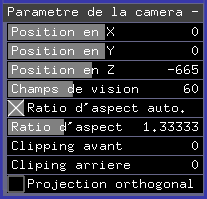
\includegraphics[width=5cm]{fig/proprieteCamera.png}
	\caption{Propriété de la caméra dans l'interface}
	\label{fig:propriete}
\end{figure}

\subsection{Mode de projection}
Le changement de mode de projection de perspective à orthogonale a été implémenté dans l'application. L'essentiel du travail se fait dans la méthode «ccamera::changeMode()». Elle est appelé lorsqu'on appuit sur le bouton à cet effet dans l'interface graphique.

\begin{lstlisting}
	if (ortho.get()) {
		cam->enableOrtho();
	} else {
		cam->disableOrtho();
	}
\end{lstlisting}

\subsection{Caméra interactive}
La caméra interactive est implémenter dans l'application principalement à l'aide de la classe ofEasyCam de openFrameworks. Nous avons tout de même ajouter la possibilité de déplacer à l'aide des flèches du clavier, pour permettre de repositionner facilement la caméra. Il est aussi possible d'avancer à caméra à l'aide de pageUp/Down. L'essentiel du code se trouve au début de «ccamera::update()».

\begin{lstlisting}
	float dist = speed * dt;
	float dx = 0;
	float dy = 0;
	float dz = 0;
	
	dx = 0;
	if (isCameraMoveLeft)
		dx += dist;
	if (isCameraMoveRight)
		dx -= dist;
	cam->truck(-dx);
	posX.set(round(-cam->getX()));
	
	dy = 0;
	if (isCameraMoveUp)
		dy -= dist;
	if (isCameraMoveDown)
		dy += dist;
	cam->boom(-dy);
	posY.set(round(cam->getY()));
	
	dz = 0;
	if (isCameraMoveForward)
		dz -= dist;
	if (isCameraMoveBackward)
		dz += dist;
	cam->dolly(dz);
	posZ.set(round(cam->getZ()));
\end{lstlisting}

\subsection{Caméra multiple}
Non-implémenté

\subsection{Caméra animée}
Non-implémenté
